\chapter{ASA Firewall Models}

\section{Introduction}

An IOS router firewall solution is appropriate for small network. The Cisco ASA provides dedicated firewall services in one device, which scales well and typically suitable for a large enterprise.\\

The ASA CLI has a similar look and feel to the Cisco router IOS. Although it shares some common features with the router IOS, it has its unique features. For example, an ASA CLI command can be executed regardless of the current configuration mode prompt. The IOS \code{do} command is not required or recognized. Different from the router IOS, the ASA provides a \code{help} command that provides a brief command description and syntax for certain commands.\\

There are two firewall modes of operation available on ASA devices: Routed and Transparent mode. In routed mode, the ASA is considered to be a router hop and supports multiple interfaces, NAT and applies policy to traffic as they transit a firewall. In transparent mode, ASA functions like a Layer 2 device and is only assigned an IP address on the local network for management purposes. In this mode, ASA does not support QoS, dynamic routing protocols, VPNs, etc.\\

The ASA assigns \textbf{security levels} to distinguish between inside and outside interfaces. The higher the level, the more trusted the interface. The security level numbers range from 0 to 100. Therefore, the interface connecting to the Internet should be assigned the lowest level. The interface connecting to the internal network should be assigned the highest level. The interface connecting to the DMZ network should be assigned a level between them.\\

When traffic moves from inside interface to outside interface, it is considered outbound traffic. Outbound traffic and return traffic (originating on the inside network) is allowed and inspected by default. Conversely, traffic moving from outside interface to inside interface is considered inbound traffic, which is denied by default. Connectivity between interfaces with the same security levels is blocked by default and only enabled by executing the \code{same-security-traffic permit inter-interface} global configuration command.\\

\section{Basic configuration on ASA 5505}

\subsection{VLAN}

With the ASA 5505, the eight integrated switch ports are Layer 2 ports. Therefore, there are two kinds of interfaces that need to be configured: Logical VLAN interfaces and Physical switch ports. \\

Logical VLAN interfaces are configured with the Layer 3 information including a name, security level, and IP address. The IP address can be configured using one of the following options: manually, DHCP, and PPPoE. 

\begin{sexylisting}{VLAN interfaces}
int vlan 1
	nameif inside
	security-level 100
	ip address 192.168.1.1 255.255.255.0
int vlan 2
	nameif outside
	security-level 100
	ip address 209.165.200.226 255.255.255.248
	exit
\end{sexylisting}

By default, all Layer 2 switch ports are assigned to VLAN 1. Therefore, we need to assign all ports connected to internal network to VLAN 1 (inside interface) and the other to VLAN 2 (outside interface). This is done using  \code{sw access vlan vlan-id} interface configuration command. \\

An ASA 5505 with a Base license does not allow three \textit{fully} functioning VLAN interfaces to be created, but a third \textit{limited} VLAN interface can be created if it is first configured with the \code{no forward interface vlan} command before the \code{nameif} command. The Security Plus license is required to have more than two VLANs with full functionality.\\

\subsection{DHCP}

The ASA 5505 Base license is a 10-user license and therefore the maximum number of DHCP clients supported is 32. To enable an ASA as a DHCP server and provide DHCP services to hosts, use the commands listed below:

\begin{sexylisting}{DHCP configuration in ASA}
dhcpd enable inside
dhcpd address 192.168.1.10-192.168.1.54 inside
dhcpd release 1800
show dhcpd ?
\end{sexylisting}

The \code{dhcpd auto-config outside} command was issued to enable the DHCP client for outside interface.

\subsection{Other configurations}

A default static route must be configured using the \code{route outside 0.0.0.0 0.0.0.0 next-hop-ip-address} command.\\

SSH is required to manage the ASA 5505 remotely, using the CLI. In the following example, AAA authentication is enabled referencing the local database, the RSA crypto key is generated using 2048 bits. Two inside hosts and an outside host are being permitted to access the ASA and SSH version 2 is enabled. The \code{aaa authentication ssh console LOCAL} command overrides the password set with the password command and authenticates the Telnet access against the local database.

\begin{sexylisting}{SSH configuration in ASA}
username ADMIN password class
aaa authentication ssh console LOCAL

crypto key generate rsa modulus 2048

ssh 192.168.1.3 255.255.255.255 inside
ssh 172.16.1.3 255.255.255.255 outside

ssh version 2
end

show ssh
\end{sexylisting}

Network Time Protocol (NTP) services can be enabled on an ASA to obtain the date and time from an NTP server. To enable NTP, use the global configuration mode commands as follow

\begin{sexylisting}{NTP in ASA}
ntp authenticate
ntp trusted-key 1
ntp authentication-key 1 md5 cisco123
ntp server 192.168.1.254
end

show ntp status
show ntp associations 
\end{sexylisting}

%
%\subsection{ASA Interactive Setup Initialization Wizard}
%
%You can erase ASA configuration using \code{write erase} and \code{reload} privileged EXEC commands. When the device is rebooted, the ASA wizard displays the prompt \textit{Pre-configure Firewall now through interactive prompts [yes]} To cancel and display the ASA default user EXEC mode prompt, enter \code{no}. Otherwise, enter \code{yes} or simply press \code{Enter}. This initiates the wizard and the ASA interactively guides an administrator to configure the default settings.
%
%\section{Basic configurations}
%
%\subsection{Setup Initialization wizard}
%
%The default ASA user prompt of \code{ciscoasa>} is displayed when an ASA configuration is erased, the device is rebooted, and the user does not use the interactive setup wizard. To enter privileged EXEC mode, use the \code{enable} user EXEC mode command. Initially, an ASA does not have a password configured; therefore when prompted, leave the enable password prompt blank and press Enter.\\
%
%The ASA date and time should be set either manually or by using Network Time Protocol (NTP). To set the date and time, use the \code{clock set} privileged EXECcommand. Enter global configuration mode using the \code{conf t} privileged EXEC command. An ASA must be configured with basic management settings. The table in Figure \ref{ASAbasic} displays the commands to accomplish this task.
%
%\begin{figure}[hbtp]
%\caption{ASA basic configuration commands}\label{ASAbasic}
%\centering
%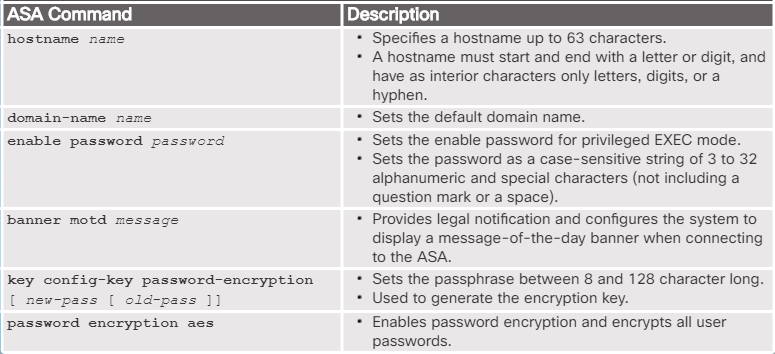
\includegraphics[scale=0.5]{pictures/ASAbasic.PNG}
%\end{figure}
%
%\subsection{Configuring Logical VLAN Interfaces}
%
%When configuring an ASA 5505, there are two kinds of interfaces that need to be configured:
%
%\begin{itemize}
%\item Logical VLAN interfaces -- These interfaces are configured with the Layer 3 information including a name, security level, and IP address.
%\item Physical switch ports -- These are Layer 2 switch ports which are assigned to the logical VLAN interfaces.
%\end{itemize}
%
%\begin{figure}[hbtp]
%\caption{Logical VLAN interface command}\label{ASAlogicalVLAN}
%\centering
%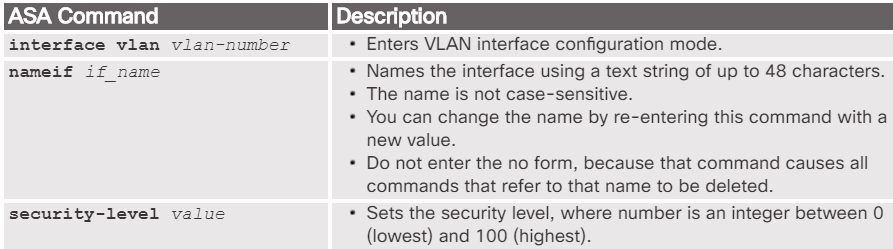
\includegraphics[scale=0.5]{pictures/ASAlogicalVLAN.PNG}
%\end{figure}
%
%
%An ASA 5505 with a Base license does not allow three fully functioning VLAN interfaces to be created. However, a third  \emph{limited} VLAN interface can be created if it is first configured with the \code{no forward interface vlan <num>} command (figure \ref{ASAlogicalVLAN}). This command limits the interface from initiating contact with another VLAN. Therefore, when the inside and outside VLAN interfaces are configured, the no forward interface vlan number command must be entered before the \code{nameif} command is entered on the third interface. The \code{<num>} argument specifies the VLAN ID to which this VLAN interface cannot initiate traffic. The Security Plus license is required to achieve full functionality.\\
%
%\subsection{Static routes and IP addresses}
%
%Switch ports on the same VLAN can communicate with each other using hardware switching. But when a switch port on VLAN 1 wants to communicate with a switch port on VLAN 2, then the ASA applies the security policy to the traffic and routes between the two VLANs. If an ASA is configured as a DHCP client, then it can receive and install a default route from the upstream device. Otherwise, a default static route must be configured using the \code{route <ifname> 0.0.0.0 0.0.0.0 next-hop-ip-address} command. To verify the route entry, use the \code{show route} command.\\
%
%The IP address of an interface can be configured using one of the following options: DHCP, PPPoE, or manually. The table in Figure \ref{SVIaddr} lists the commands to configure an IP address on an interface. 
%
%\begin{figure}[hbtp]
%\caption{Configure IP addresses on logical VLAN interfaces}\label{SVIaddr}
%\centering
%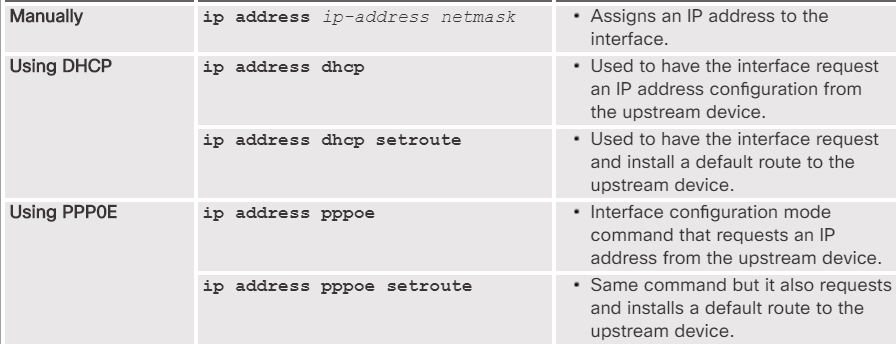
\includegraphics[scale=0.5]{pictures/SVIaddr.PNG}
%\end{figure}
%
%\subsection{Remote access}
%
%\begin{figure}[hbtp]
%\caption{ASA Telnet configuration commands}\label{TelnetConfigASA}
%\centering
%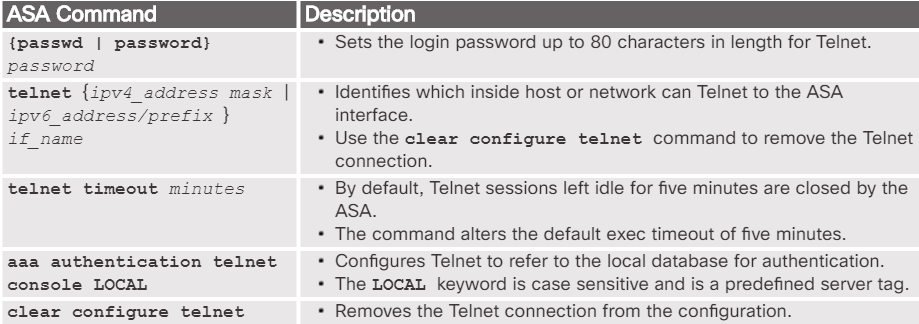
\includegraphics[scale=0.5]{pictures/TelnetConfigASA.PNG}
%\end{figure}
%
%\begin{figure}[hbtp]
%\caption{Sample ASA Telnet configuration}\label{TelnetExample}
%\centering
%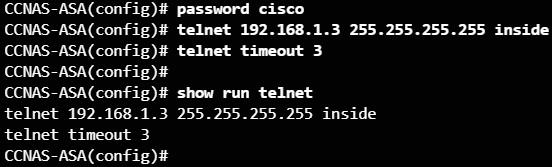
\includegraphics[scale=0.5]{pictures/TelnetExample.PNG}
%\end{figure}
%
%
%\begin{figure}[hbtp]
%\caption{ASA ssh configuraiton commands}\label{SSHconfigASA}
%\centering
%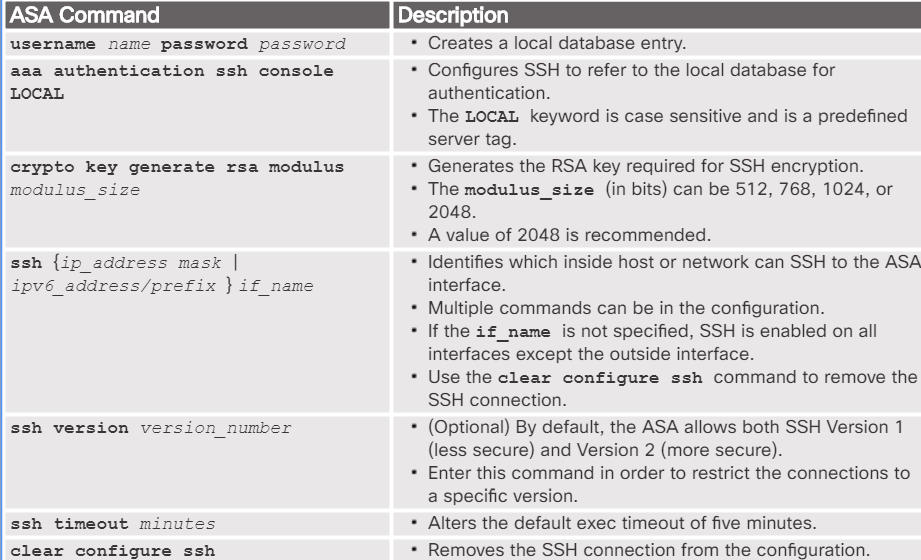
\includegraphics[scale=0.5]{pictures/SSHconfigASA.PNG}
%\end{figure}
%
%\subsection{NTP configuration}
%
%\begin{figure}[hbtp]
%\caption{NTP authentication commands}
%\centering
%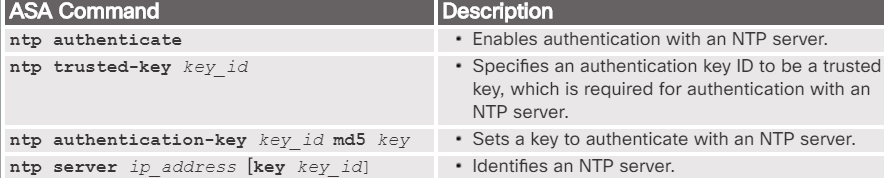
\includegraphics[scale=0.5]{pictures/NTPauthentication.PNG}
%\end{figure}
%
%\subsection{DHCP configuration}
%
%\begin{figure}[hbtp]
%\caption{DHCP server commands}\label{DHCPcommandList}
%\centering
%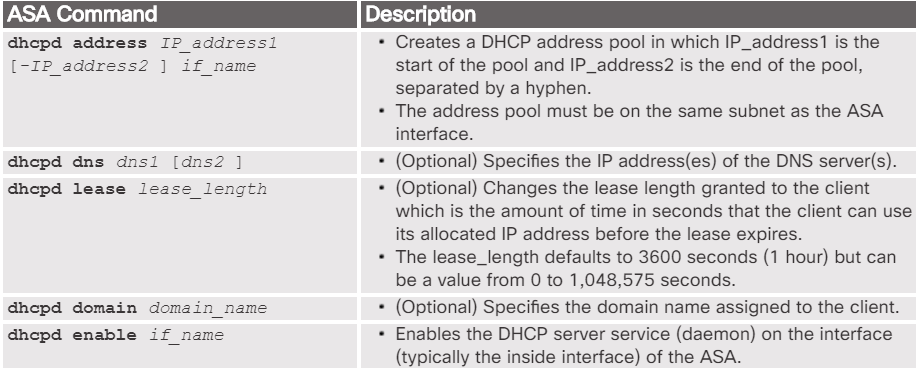
\includegraphics[scale=0.5]{pictures/DHCPcommandList.PNG}
%\end{figure}
%
%
%The example in Figure \ref{DHCPcommand} enables the DHCP service for inside clients on an ASA 5505. The ASA 5505 Base license can provide IP configuration information for up to 32 DHCP clients. If the ASA outside interface was configured as a DHCP client, then the \code{dhcpd auto outside} global configuration mode command can be used to pass the DHCP-obtained information to the DHCP inside clients.
%
%\begin{figure}[hbtp]
%\caption{Sample configuration ASA as an DHCP server}\label{DHCPcommand}
%\centering
%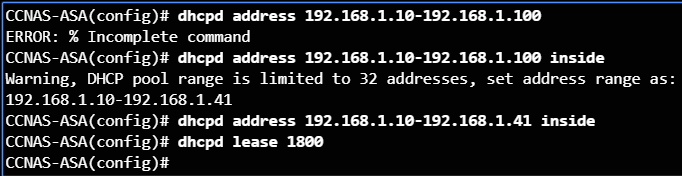
\includegraphics[scale=0.5]{pictures/DHCPcommand.PNG}
%\end{figure}

\section{Objects and Object Groups}

An object can be a particular IP address, an entire subnet, a range of addresses, a protocol, or a specific port or range of ports. In other words, defining object is similar to defining variables in programming. There are two types of objects that can be configured:

\begin{itemize}
\item Network object: a single IP address and subnet mask and there are three types: host, subnet, or range. A network object is configured using the \code{object network <name>} command.
\item Service object: a protocol and optional source and/or destination port. A service object is configured using the \code{object service <name>} command.
\end{itemize}

\note Note: A network object is required to configure NAT in ASA image versions 8.3 and higher.

\subsection{Network object}

There can only be one statement in the network object. Entering a second IP address/mask pair replaces the existing configuration. To erase all network objects, use the clear config object network command. 

\begin{sexylisting}{Network object}
object network ADMIN-HOST
	host 192.168.1.3
	exit
object network INTERNAL
	subnet 192.168.1.0 255.255.255.224
	exit
object network PUBLIC-ADDR
	range 209.165.200.240 209.165.200.248
	exit
show run object	network
\end{sexylisting}

\subsection{Service object}

A service object name can only be associated with one protocol and port (or ports). If an existing service object is configured with a different protocol and port, the new configuration replaces the existing protocol and port with the new ones. 

\begin{sexylisting}{Service object}
object service WEB
	service tcp destination eq ftp
	service tcp destination eq www
	exit
show run object service	
\end{sexylisting}

\subsection{Object group}

Objects can be grouped together to create an object group. By grouping like objects together, an object group can be used in an access control entry (ACE) instead of having to enter an ACE for each object separately.

\note  A network object group cannot be used to implement NAT. A network object is required to implement NAT.

\begin{sexylisting}{Network object group}
object network LEAD-ADMIN
	host 192.168.1.3
	exit
object-group network ADMIN-HOST
	description Administrative hosts
	network-object LEAD-ADMIN
	network-object host 192.168.1.4
	exit
object-group network INSIDE
	description All inside hosts
	network-object host 192.168.1.32 255.255.255.240
	group-object ADMIN-HOST
	exit
show run object-group		
\end{sexylisting}

\begin{sexylisting}{ICMP object group}
object-group icmp-type ICMP-ALLOWED
	icmp-object echo
	icmp-object time-exceeded
	exit
\end{sexylisting}

\begin{sexylisting}{Service object group}
object-group service WEB-PAGE
	service-object tcp destination www
	service-object tcp destination https
	exit
object-group service MAIL tcp
	port-object eq www
	port-object eq smtp
	exit	
object-group service DOWNLOAD
	group-object MAIL
	port-object eq ftp
	port-object range 2000 2005
	exit	
\end{sexylisting}


\section{ACL in ASA}

ASA standard ACLs are used to identify the destination IP addresses, unlike IOS ACLs where a standard ACL identifies the source host/network. They are typically only used for OSPF routes and can be used in a route map for OSPF redistribution. Standard ACLs cannot be applied to interfaces to control traffic.\\

ASA ACLs use the subnet mask in defining a network, whereas IOS ACLs use the wildcard mask.\\

The ASA supports five types of access lists: Extended, Standard, EtherType, WebType, and IPv6 access lists. An EtherType ACL can be configured only if the security appliance is running in transparent mode. The Webtype ACLs are used in a configuration that supports filtering for clientless SSL VPN users.\\

\begin{sexylisting}{Simple ACL in ASA}
access-list ACL-IN extended permit ip 192.168.1.0 255.255.255.0 209.165.201.0 255.255.255.24
access-group ACL-IN in interface inside
\end{sexylisting}

\begin{sexylisting}{ACL with object groups}
object-group network NET-HOSTS
	network-object host 209.165.201.1
	network-object host 209.165.201.2
	exit
object-group network SERVERS
	network-object host 209.165.202.131
	network-object host 209.165.202.132
	exit
object-group service HTTP-SMTP tcp
	port-object eq smtp
	port-object eq www
	exit
access-list ACL-IN extended permit tcp object-group NET-HOSTS object-group SERVERS object-group HTTP-SMTP
\end{sexylisting}

\section{NAT in ASA}

Besides normal form of NAT (dynamic NAT, static NAT, PAT), ASA also supports Policy NAT. This kink of NAT is based on a set of rules. These rules can specify that only certain source addresses intended for specific destination addresses and/or specific ports will be translated. For example, policy NAT would be used on an ASA where 10.0.1.0/24 inside addresses are to be translated only if traffic from these addresses is destined for the 198.133.219.0/24 network.\\

NAT can be deployed on an ASA using one of these methods:

\begin{itemize}
\item inside NAT: when a host from a higher-security interface has traffic destined for a lower-security interface and the ASA translates the internal host address to a global address
\item outside NAT: when traffic from a lower-security interface destined for a host on the higher-security interface is translated
\item bidirectional NAT: when both inside NAT and outside NAT are used together
\end{itemize}

To configure network object dynamic NAT, two network objects are required. A network object identifying the pool of public IP addresses. The other identifies the internal addresses to be translated and then binds the two objects together. Use the \code{show xlate} and \code{show nat detail} commands to verify translations.\\

\begin{sexylisting}{Dynamic NAT in ASA}
object network PUBLIC
	range 209.165.200.240 209.165.200.248
	exit
object network DYNAMIC-NAT
	subnet 192.168.1.0 255.255.255.224
	nat (inside,outside) dynamic PUBLIC
	exit
show xlate
show nat detail	
\end{sexylisting}

When configuring Dynamic PAT, Only one network object is required when overloading the outside interface. 

\begin{sexylisting}{PAT in ASA}
object network INSIDE-NET
	subnet 192.168.1.0 255.255.255.224
	nat (inside,outside) dynamic interface
\end{sexylisting}

Static NAT is configured when an inside address is mapped to an outside address. For instance, static NAT can be used when a server must be accessible from the outside. 

\begin{sexylisting}{Static NAT in ASA}
object network DMZ-SERVER
	host 192.168.2.3
	nat (dmz,outside) static 209.165.200.227
	exit
	
access-list OUTSIDE-DMZ extended permit ip any host 192.168.2.3
access-group OUTSIDE-DMZ in interface outside

access-list ICMPACL extended permit ip any any
access-group ICMPACL in interface dmz

policy-map global_policy
	inspect inspection_default
\end{sexylisting}


\section{AAA in ASA}

To create a TACACS+ or RADIUS server, use the commands listed below:

\begin{sexylisting}{Create authentication server in ASA}
aaa-server TACACS-SEVER protocol tacacs+
	aaa-server TACACS-SEVER (dmz) host 192.168.2.3
	exit
\end{sexylisting}

To authenticate users who access the ASA CLI over a console, SSH, HTTPS (ASDM), or to authenticate users who access privileged EXEC mode using the following command.

\begin{sexylisting}{Authenticate users}
aaa authentication http console TACACS-SERVER LOCAL
aaa authentication enable console TACACS-SERVER LOCAL
aaa authentication ssh console TACACS-SERVER LOCAL
\end{sexylisting}


\section{Modular Policy Framework (MPF)}

A Modular Policy Framework (MPF) configuration defines a set of rules for applying firewall features, such as traffic inspection and QoS. There are three configuration objects in the MPF; class maps, policy maps, and service policy. The class maps configuration object uses match criteria to identify interesting traffic.\\

There are four steps to configure MPF on an ASA:

\begin{itemize}
\item Configure extended ACLs to identify granular traffic that can be specifically referenced in the class map. For example, ACLs can be used to match TCP traffic, UDP traffic, HTTP traffic, or all traffic to a specific server.

\item Configure the class map to identify traffic (figure \ref{classmap}.

\item Configure a policy map to apply actions to those class maps.

\item Configure a service policy to attach the policy map to an interface.
\end{itemize}

\begin{figure}[hbtp]
\caption{Configure the class map to identify traffic}\label{classmap}
\centering
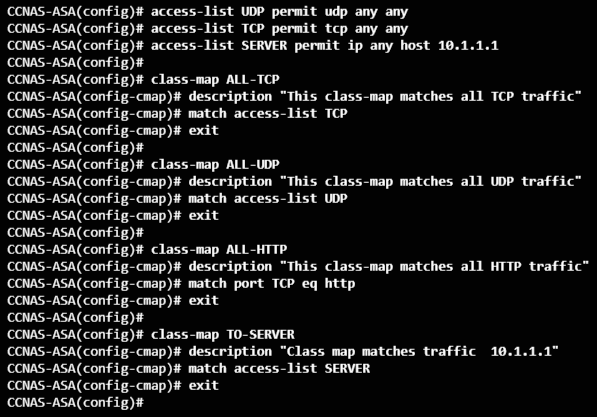
\includegraphics[scale=0.7]{pictures/classmap.PNG}
\end{figure}

The names \code{class-default} and any name that begins with \verb|_internal| or \verb|_default| are reserved. The class map name must be unique and can be up to 40 characters in length.\\

The ASA also automatically defines a default Layer 3/4 class map identified in the configuration by \verb|class-map inspection_default|. Identified in this class map is the \code{match default-inspection-traffic} which matches the default ports for all inspections. When used in a policy map, this class map ensures that the correct inspection is applied to each packet, based on the destination port of the traffic.

Policy maps are used to bind class maps with actions (figure \ref{MPFimplementation}). The default configuration includes a default Layer 3/4 policy map is called \verb|global_policy| (figure \ref{DefaultPolicy}). This policy performs an inspection on the default inspection traffic. There can only be one global policy. Therefore, to alter the global policy, either edit it or replace it.

\begin{figure}[hbtp]
\caption{Create policy map for MPF}\label{MPFimplementation}
\centering
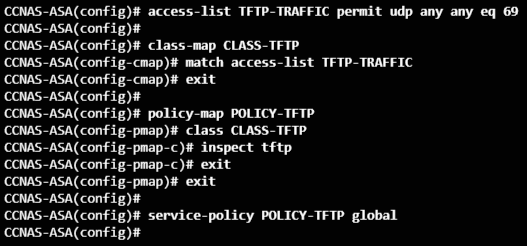
\includegraphics[scale=0.7]{pictures/MPFimplementation.PNG}
\end{figure}

\begin{figure}[hbtp]
\caption{Default service policy configuration}\label{DefaultPolicy}
\centering
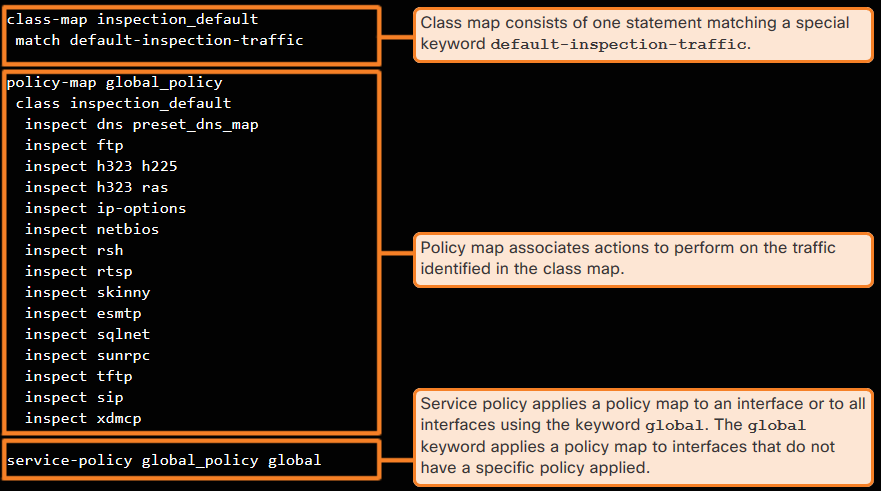
\includegraphics[scale=1]{pictures/DefaultPolicy.PNG}
\end{figure}
